\newpage
\chapter{Background}

\section{Argumentation}
Argumentation in general involves studying how claims and conclusions can be reached by applying logical reasoning.  It is useful when analysing arguments in the form of dialogue and persuasion, especially under the context of philosophy, medicine and law. Research in artificial intelligence is looking to exploit the underlying logic in analysing arguments to allow for this analysis to be carried out in a computerised manner. In order to do so general purpose argumentation frameworks have been devised to allow for analysis of an argument as a computerised argumentation problem. Two such argumentation frameworks are Abstract Argumentation (AA) and Assumption-Based Argumentation (ABA). Argumentation frameworks such as these can provide the general basis required to implement specific frameworks for real-life problems where argumentation could help in decision making and argument analysis. For the web-based application proposed by this project the underlying framework will be ABA.

\section{Assumption-Based Argumentation}
Although ABA is an instance of AA, there are core differences in the way ABA perceives and evaluates arguments. In ABA arguments and attacks are derived from given rules in a deductive system, assumptions and their contraries \cite{abatut}. An argument is supported by assumptions and is attacked by other arguments when the contrary of an assumption of the initial argument can be deduced by the opposing argument. However, in order for an argument to be deemed ``acceptable'' or ``winning'', ABA is equipped with numerous semantics that allow us to determine an ``acceptable/winning'' set of assumptions, from which we can deduce an ``acceptable'' set of arguments.  Additionally several computational mechanism have been developed for ABA (see \cite{proxdd} and \cite{grapharg}) that allow a conclusion or claim to be algorithmically evaluate in terms of a ``acceptable'' set of arguments. The computational nature of these mechanisms allow us to programmatically implement the semantics and allow for computerised argumentation analysis of a framework.

\section{The ABA framework}
The potential power of ABA lies with its ability to represent and evaluate real-world decision problems. An implementation of ABA could prove to be an invaluable tool when it comes to evaluating potential claims, providing support to existing claims or disputing existing claims, in any context as long as it can be generalised and implemented as part of the ABA framework.

The following is an example taken from \cite{abatut} to demonstrate how ABA can interpret a simple real-world problem, while introducing the ABA framework and its elements.

``You like eating food, this makes you really happy. But you are very health-conscious too, and don't want to eat without a fork and with dirty hands. You are having a walk with some friends, and your friend Nelly is offering you all a piece of lasagne, looking really delicious. You are not quite sure, but typically you carry no cutlery when you go for walks, and your hands will almost certainly be dirty even if the may not look so. Should you go for the lasagne, trying to snatch it quickly from the other friend? You may argue with yourself as follows:

\ensuremath{\alpha} : let me go for the lasagne, it looks delicious, and eating it will make me happy!

\ensuremath{\beta} : but I am likely to have no fork and my hands will be dirty, I don't want to eat it in these circumstances, let the others have it!

\ensuremath{\alpha} and \ensuremath{\beta} can be seen as arguments, and \ensuremath{\beta} disagrees with (attacks) \ensuremath{\alpha}. If these are all the arguments put forward, since no argument is proposed that defends \ensuremath{\alpha} against \ensuremath{\beta} , the decision to go for the lasagne is not dialectically justified. If, however, you put forward the additional argument

\ensuremath{\gamma} : who cares about the others, let me get the lasagne, I may have a fork after all …

This provides a defence for \ensuremath{\alpha} against \ensuremath{\beta}, and the decision to go for the lasagna becomes dialectically (although possibly not ethically) justified.''

This example is illustrative of the breadth of problems that could potentially be analysed by an ABA system. Granted the example is overly simplistic. It has a limited amount of arguments and accounts for just a few of the possible parameters that could affect whether we are happy or not. Nonetheless, being a general framework the simplicity of the problem does not affect our ability to device a specific framework for this problem from which we can evaluate our claim of being happy (or not being happy). 

The ABA frame work is defined by \cite{abatut} as follows:

\begin{defn}
An ABA framework is a tuple $\langle\mathcal{L}$, $\mathcal{R}$, $\mathcal{A}$, {\bf\textasciimacron} $\rangle$ where
\begin{itemize*}
	\item $\langle\mathcal{L}$, $\mathcal{R}\rangle$ is a deductive system, with $\mathcal{L}$ the \emph{language} and $\mathcal{R}$ a set of \emph{rules}, that we assume of the form $\sigma_0 \leftarrow \sigma_1, \ldots, \sigma_m (m \geq 0)$ with $\sigma_i \in \mathcal{L} (i = 0, \ldots, m)$; $\sigma_0$ is referred to as the \emph{head} and $\sigma_i, \ldots, \sigma_m $  as the \emph{body} of the rule $\sigma_0 \leftarrow \sigma_1, \ldots, \sigma_m $ ;
	\item $\mathcal{A}\subseteq\mathcal{L}$ is a (non-empty) set, referred to as \emph{assumptions};
	\item {\bf\textasciimacron} is a total mapping from $\mathcal{A}$ into $\mathcal{L}$; $\bar{\alpha}$ is referred to as the \emph{contrary} of $\alpha$.
	
\end{itemize*}
\end{defn}

Referring back to the example used let us assume that the following mapping exists:

\begin{multicols}{2}
\begin{itemize*}

\item \it{p} - happy
\item \it{r} - not happy
\item \it{a} - eating
\item \it{q} - good food
\item \it{b} - no fork
\item \it{c} - dirty hands
\item \it{s} - fork
\item \it{t} - clean hands

\end{itemize*}
\end{multicols}

Based on this mapping and the definition of the an ABA framework we can now construct a framework that represents the example, as shown in \cref{exmp_1}:

\begin{exmp}\label{exmp_1}
$\langle\mathcal{L}$, $\mathcal{R}$, $\mathcal{A}$, {\bf\textasciimacron} $\rangle$ may consist of

$\mathcal{L} = \{a,b,c,p,q,r,s,t\}$

$\mathcal{R} = \{p \leftarrow q,a, q \leftarrow, r \leftarrow b,c \}$

$\mathcal{A} = \{a, b, c\}$

$\bar{a} = r, \bar{b} = s, \bar{c} = t $

\end{exmp}

The framework constructed in \cref{exmp_1} displays the various elements that allow one to represent a real-life decision problem in ABA. It can be seen that the rules related to our problem are defined in terms of inference rules. Additionally, the framework also includes the following elements:

\begin{description}

\item[Assumptions] are, in our example, actions that can be taken or disputable observations about the argument. In general assumptions can be considered as vulnerable points of an argument that can be used to support or dispute that argument. The aim of ABA is to establish a set of ``strong'' assumptions that support or dispute the underlying argument.
\item[Non-Assumptions] represent goals we wish to achieve or avoid in accordance to the claim we are trying to analyse. These can be based on certain assumption we are considering or might be stand-alone goals.
\item[Contraries] are sentences that are opposing to the assumptions of our framework. ABA imposes that each assumption must be mapped to a contrary. For example, the assumption ``no fork'' in our framework has a contrary of ``fork''. Thus our framework is now equipped with both the assumptions necessary but also the opposing assumptions that can dispute them.

\end{description}

The description provides a simple overview of what these elements of the framework are and are used in the example. This will allow us to explore how claims are analysed. For the purpose of this report there is no need to explore to a deeper level the framework, however there are numerous publications that explain in these elements in more detail (see \cite{abatut}).

\section{Proving a claim using ABA}
The ability of ABA to evaluate the support of a claim, lies in its ability to formulate and analyse arguments. Arguments are the deduction of a certain claim from the rules and assumptions provided. The following is a definition of an argument (according to \cite{abatut}):
\newline

\begin{defn} an argument is defined as follows:

An argument for (the claim) $\sigma \in \mathcal{L}$ supported by $A \subseteq \mathcal{A}$ $(A \vdash \sigma$ in short) is a deduction for $\sigma$ supported by A (and some R $\subseteq \mathcal{R})$
\newline
\end{defn}


However, within the ABA framework there is also the notion of attack (similarly to AA). An attack between arguments under ABA occurs when one argument deduces the contrary of an assumption of another argument. 
Attacks can be defined as follows (from \cite{abatut}):
\newline

\begin{defn} an attack is defined as follows:

An argument $A_1 \vdash \sigma_1$ attacks an argument $A_2 \vdash \sigma_2$ iff $\sigma_1$ is the contrary of one of the assumptions in $A_2$.
\newline
\end{defn}

ABA is equipped with various semantics that allow it to determine ``winning/acceptable'' sets of arguments and assumptions. This enables us to validate whether a claim can be deduced from these ``acceptable'' arguments and whether the claim is supported by these ``winning'' assumptions. These semantics can define the ``acceptability'' of both a set of arguments and a set of assumptions. Both approaches (or views) are defined below (in accordance to \cite{abatut}):
\newline

Argument View Semantics
\begin{itemize*}
\item \emph{admissible} iff it does not attack itself and it attacks all arguments that attack it;
\item \emph{preferred} iff it is maximally (w.r.t. $\subseteq$) admissible;
\item \emph{sceptically preferred} iff it is the intersection of all preferred sets of arguments;
\item \emph{complete} iff it is admissible and contains all arguments it \emph{defends}, where A defends $\alpha$ iff A attacks all arguments that attack $\alpha$;
\item \emph{grounded} iff it is minimally (w.r.t $\subseteq$) complete;
\item \emph{ideal} iff it is maximally (w.r.t $\subseteq$) admissible \emph{and} contained in all preferred sets of arguments;
\item \emph{stable} iff it does not attack itself and it attacks all arguments it does not contain.
\end{itemize*}

Assumption View Semantics
\begin{itemize*}
\item \emph{admissible} iff it does not attack itself and it attacks all assumptions that attack it;
\item \emph{preferred} iff it is maximally (w.r.t. $\subseteq$) admissible;
\item \emph{sceptically preferred} iff it is the intersection of all preferred sets of assumptions;
\item \emph{complete} iff it is admissible and contains all assumptions it \emph{defends}, where A defends $\alpha$ iff A attacks all assumptions that attack $\alpha$;
\item \emph{grounded} iff it is minimally (w.r.t $\subseteq$) complete;
\item \emph{ideal} iff it is maximally (w.r.t $\subseteq$) admissible \emph{and} contained in all preferred sets of assumptions;
\item \emph{stable} iff it does not attack itself and it attacks all assumptions it does not contain.
\end{itemize*}

\section{Computational mechanisms for ABA}
The power of ABA is unleashed through the various computational mechanisms and tools that have been developed. These allow for ABA frameworks to be analysed in an algorithmic manner, thus allowing the creation of computerised systems that can carry out this analysis. The underlying features of these mechanisms are as follows (as described by \cite{abatut}):
\newline

\begin{itemize*}
\item they can be abstracted away as disputes between a \emph{proponent} and an \emph{opponent}, in a sort of (fictional) zero-sum, two-player game: the proponent aims at proving (constructively) that an initially given \emph{sentence} is ``acceptable''/``winning'', the opponent is trying to prevent the proponent from doing so;
\item these disputes are defined as a \emph{sequence of tuples} (referred to as \emph{dispute derivations}), representing the state of the game while it is being played;
\item these disputes interleave the construction of arguments and identification of attacks between them with testing whether the input sentence is ``acceptable''/``winning'';
\item the rules of the game allow proponent and opponent to perform various kinds of \emph{filtering} during disputes, but different kinds for different argumentation semantics (for determining whether the input sentence is ``acceptable''/``winning'';
\item the possible outcomes of dispute derivations are as follows:
\begin{itemize*}
\item the input sentence is proven to be ``acceptable''/``winning'' (the dispute derivation is \emph{successful}) or is not proven to be so; and
\item if the dispute derivation is successful, it returns:
\begin{enumerate*}
\item the set of all assumptions supporting the arguments by the proponent(referred to as the \emph{defence set}),
\item the set of all assumptions in the support of arguments by the opponent and chosen by the proponent to be counter-attacked (referred to as the \emph{culprits}),
\item in the case of the proposal of (\cite{proxdd}), the \emph{dialectical tree} of arguments by proponent and opponent.
\end{enumerate*}
\end{itemize*}
\end{itemize*}

With these features in mind several procedure and algorithms have been devised that determine whether a claim is ``acceptable/winning'' based on several of the semantics mentioned. These include a wide range of tools from flowcharts to logic programming systems, some of which are discussed in the following sections.

\section{Proxdd} \label{subsec:proxdd}
Proxdd (refer to \cite{proxddsys}) is a system developed by Dr. Robert Craven that implements dispute derivations to analyse ABA frameworks. Given a constructed framework it can algorithmically analyse and return a set of winning arguments in accordance to the semantics specified. Proxdd currently supports admissible and grounded semantics. It is implemented using the Prolog logic programming language (for more details see \cite{proxddsys}). The underlying computational mechanism used for Proxdd is the SXDD algorithm (defined in \cite{proxdd}).

\begin{exmp} Example of input (from \cite{proxddsys}) \label{graph_in}
\begin{verbatim}
myAsm(a). 
myAsm(b). 
myAsm(c). 
myAsm(d). 
myAsm(e). 
myAsm(f). 
contrary(a, q). 
contrary(b, f). 
contrary(c, u). 
contrary(d, v). 
contrary(e, v). 
contrary(f, v). 
myRule(p, [a,u]). 
myRule(q, [b,r]). 
myRule(q, [c,s]). 
myRule(q, [c,t]).
myRule(u, [a]). 
myRule(s, []). 
myRule(t, [d]). 
myRule(t, [e]). 
\end{verbatim}
\end{exmp}

\begin{exmp} Example of output (from \cite{proxddsys})
\begin{verbatim}
DEF:	[a] 
CUL:	[c]
ARG:	[1:([a], [] -> p),6:([c], [] -> q),7:([a], [] -> u), 
		 8:([c], [d] -> q),9:([c], [e] -> q)] 
ATT:	[1-0,6-1,7-6,8-1,9-1] 
\end{verbatim}
\end{exmp}

\section{Grapharg} \label{subsec:grapharg}
Grapharg (refer to \cite{graphargsys}) is a system also developed by Dr. Robert Craven. Similarly to Proxdd it also provides dispute derivation for ABA. Furthermore, it is also implemented in Prolog, however the underlying algorithm is different. Unlike Proxdd it uses a graph-based dispute derivation algorithm that, according to the research's findings, optimises the computation of the dispute derivation (refer to \cite{grapharg}).

In both Proxdd and Grapharg the system takes in a framework in the form shown in \cref{graph_in} and after the dispute derivation it produces an output similar to \cref{exmp_graph}. Additionally, by using graphviz, the output can be displayed graphically as in \cref{exmp_graphimg}. 
\newline

\begin{exmp} Example of output (from \cite{graphargsys}) \label{exmp_graph}
\begin{verbatim}
DEFENCE:	[a]
CULPRITS:	[c]
PROP JUSTIFICATIONS:	[(a,*),(p,1),(u,5)]
OPP JUSTIFICATIONS:	[[]-[(c,*),(d,*),(q,4),(t,7)]-[q],
					[]-[(c,*),(e,*),(q,4),(t,8)]-[q],[]-[(c,*),
					(q,3),(s,6)]-[q]]
ATTACKS:	[(q,a),(u,c)]
GRAPH:	[]
\end{verbatim}

\end{exmp}

\begin{exmp} Example of current visualisation using graphviz (from \cite{graphargsys}) \label{exmp_graphimg}

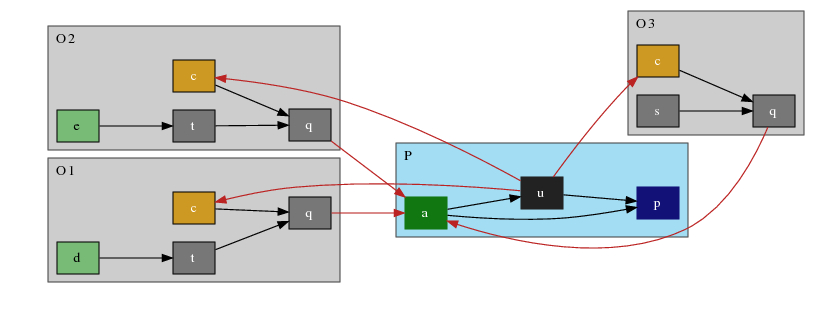
\includegraphics[width=\linewidth]{graphviz}

\end{exmp}

However these systems are not user-friendly enough to promote ABA as an easily accessible tool. Both systems require setting up and both are operated using Prolog which many users might not be comfortable with. This means that the systems are not readily accessible to users and the interface provided could be more useful. This project aims at creating a web-application that will enable users to easily and instantly interact with the systems in an online and more user-friendly environment.

\section{ASPARTIX}
Perhaps the system that best resembles the desirable outcome of the project in terms of user experience and design is the ASPARTIX system (see \cite{aspartix}). ASPARTIX offers a web-application implementation that enables a user to enter a series of arguments and attack relationships between the arguments (see \cref{exmp_aspartixin}), which is then processed and displayed diagrammatically to the user (see \cref{exmp_aspartixout}).  Our implementation should aim at providing a similar experience; allowing the user to implement their framework and displaying the results diagrammatically. However, ASPARTIX does not implement ABA instead it focuses more on Abstract Argumentation. Nonetheless, elements of the system such as its implementation as a web-application, the user's ability to define a framework and the existence of a canvas on which the visualisation is displayed will have to be integrated in this project's web-application as well.

\begin{exmp} Example of input in ASPARTIX (from \cite{aspartixsys}) \label{exmp_aspartixin}
\begin{verbatim}
arg(peter).
arg(paul).
arg(christina).
att(christina, paul).
att(peter, christina).
att(paul, peter).                  
\end{verbatim}
\end{exmp}

\begin{exmp} Example of visualisation of ASPARTIX (from \cite{aspartixsys}) \label{exmp_aspartixout}

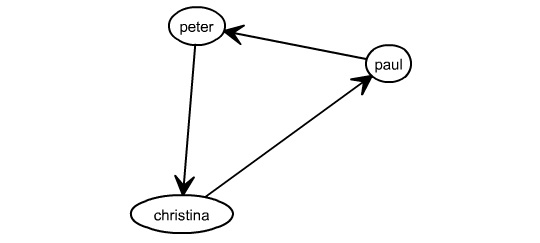
\includegraphics[width=\linewidth]{aspartix}

\end{exmp}

\section{Implementing Ideal semantics dispute derivations} \label{subsec:ideal}
Both Proxdd and Grapharg currently do not support analysing ABA according to ideal semantics. Nonetheless, the computational mechanisms do exist (see \cite{idealsem}). By extending the engines with this additional computational mechanism, we will allow our web-application to provide analysis under the ideal semantics with minimal additional development effort. 

Essentially this form of dispute derivation is an adapted version of that of the admissible semantics. Formally it is defined as follows (according to \cite{idealsem}):
\newline

\begin{defn} \label{def_fail} Let $\langle\mathcal{L}$, $\mathcal{R}$, $\mathcal{A}$, {\bf\textasciimacron} $\rangle$ be an assumption based framework. Given a selection function, an \emph{IB-dispute derivation of an ideal support} A for a sentence $\alpha$ is a finite sequence of tuples
\newline

$\langle\mathcal{P}_0, \mathcal{O}_0, A_0, \mathcal{C}_0, \mathcal{F}_0 \rangle,\ldots, \langle\mathcal{P}_i, \mathcal{O}_i, A_i, \mathcal{C}_i, \mathcal{F}_i \rangle, \ldots, \langle\mathcal{P}_n, \mathcal{O}_n, A_n, \mathcal{C}_n, \mathcal{F}_n \rangle$

where

\begin{multicols}{3}
$\mathcal{P}_0=\{\alpha\}$

$\mathcal{P}_n=\mathcal{O}_n=\mathcal{F}_n=\{\}$

\columnbreak

$\mathcal{A}_0=\mathcal{A} \cap \mathcal{P}_0$

$A=A_n$

\columnbreak

$\mathcal{O}_0=\mathcal{C}_0=\mathcal{F}_0=\{\}$

\end{multicols}

and for every $0 \leq i < n$, only one $\sigma$ in $\mathcal{P}_i$ or one S in $\mathcal{O}_i$ or one S in $\mathcal{F}_i$ is selected, and:
\\
\begin{enumerate}
\item If $\sigma \in \mathcal{P}_i$ is selected then
\begin{enumerate}
\item if $\sigma$ is an assumption then

\begin{multicols}{3}
$\mathcal{P}_{i+1}=\mathcal{P}_i - \{\sigma\}$

$\mathcal{O}_{i+1}=\mathcal{O}_i \cup \{\{\bar{\sigma}\}\}$

\columnbreak

$A_{i+1}=A_i$

$\mathcal{F}_{i+1}=\mathcal{F}_i$

\columnbreak

$\mathcal{C}_{i+1}=\mathcal{C}_i$

\end{multicols}
\item if $\sigma$ is not an assumption, then there exists some inference rule $\sigma \leftarrow R \in \mathcal{R}$ such that $\mathcal{C}_i \cap R=\{\}$ and

\begin{multicols}{3}
$\mathcal{P}_{i+1}=\mathcal{P}_i - \{\sigma\} \cup (R-A_i)$

$\mathcal{O}_{i+1}=\mathcal{O}_i$

\columnbreak

$A_{i+1}=A_i \cup (A \cap R)$

$\mathcal{F}_{i+1}=\mathcal{F}_i$

\columnbreak

$\mathcal{C}_{i+1}=\mathcal{C}_i$

\end{multicols}
\end{enumerate}
\item If S is selected in $\mathcal{O}_i$ then $\sigma$ is selected in $S_u$ and
\begin{enumerate}
\item if $\sigma$ is an assumption, then
\begin{enumerate}
\item either $\sigma$ is ignored, i.e.
\begin{multicols}{3}
$\mathcal{O}_{i+1}=\mathcal{O}_i-\{S\}\cup\{m(\sigma,S)\}$

$\mathcal{C}_{i+1}=\mathcal{C}_i$

\columnbreak

$\mathcal{P}_{i+1}=\mathcal{P}_i$

$\mathcal{F}_{i+1}=\mathcal{F}_i$

\columnbreak

$A_{i+1}=A_i$

\end{multicols}
\item or $\sigma \notin A_i$ and $\sigma \in \mathcal{C}_i$ and
\begin{multicols}{3}
$\mathcal{O}_{i+1}=\mathcal{O}_i-\{S\}$

$\mathcal{C}_{i+1}=\mathcal{C}_i$

\columnbreak

$\mathcal{P}_{i+1}=\mathcal{P}_i$

$\mathcal{F}_{i+1}=\mathcal{F}_i \cup \{u(S)\}$

\columnbreak

$A_{i+1}=A_i$

\end{multicols}
\item or $\sigma \notin A_i$ and $\sigma \notin \mathcal{C}_i$ and
\begin{enumerate}
\item if $\bar{\sigma}$ is not an assumption, then
\begin{multicols}{3}
$\mathcal{O}_{i+1}=\mathcal{O}_i-\{S\}$

$\mathcal{C}_{i+1}=\mathcal{C}_i \cup \{\sigma\}$

\columnbreak

$\mathcal{P}_{i+1}=\mathcal{P}_i \cup \{\bar{\sigma}\}$

$\mathcal{F}_{i+1}=\mathcal{F}_i \cup \{u(S)\}$

\columnbreak

$A_{i+1}=A_i$

\end{multicols}
\item if $\bar{\sigma}$ is an assumption, then
\begin{multicols}{3}
$\mathcal{O}_{i+1}=\mathcal{O}_i-\{S\}$

$\mathcal{C}_{i+1}=\mathcal{C}_i \cup \{\sigma\}$

\columnbreak

$\mathcal{P}_{i+1}=\mathcal{P}_i$

$\mathcal{F}_{i+1}=\mathcal{F}_i \cup \{u(S)\}$

\columnbreak

$A_{i+1}=A_i \cup \{\bar{\sigma}\}$

\end{multicols}
\end{enumerate}
\end{enumerate}
\item if $\sigma$ is not an assumption, then
\begin{multicols}{3}
$\mathcal{P}_{i+1}=\mathcal{P}_i$

$A_{i+1}=A_i$

$\mathcal{C}_{i+1}=\mathcal{C}_i$
\end{multicols}
$\mathcal{F}_{i+1}=\mathcal{F}_i\cup\{S-\{\sigma\}\cup R | \sigma \leftarrow R \in \mathcal{R}$ and $R \cap \mathcal{C}_i \neq \{\}\}$

$\mathcal{O}_{i+1}=\mathcal{O}_i-\{S\}\cup \{S-\{\sigma\} \cup R | \sigma \leftarrow R \in \mathcal{R}$ and $R \cap \mathcal{C}_i=\{\}\}$
\end{enumerate}
\item If S is selected in $\mathcal{F}_i$ then \emph{Fail(S)} and 
\begin{multicols}{3}
$\mathcal{O}_{i+1}=\mathcal{O}_i$

$\mathcal{C}_{i+1}=\mathcal{C}_i$

\columnbreak

$\mathcal{P}_{i+1}=\mathcal{P}_i$

$\mathcal{F}_{i+1}=\mathcal{F}_i-\{S\} $

\columnbreak

$A_{i+1}=A_i $

\end{multicols}
\end{enumerate}

\end{defn}

Fail(S) is computed as follows:
\begin{defn} Let $\langle\mathcal{L}$, $\mathcal{R}$, $\mathcal{A}$, {\bf\textasciimacron} $\rangle$ be an assumption based framework. Given a selection function, a \emph{Fail-dispute derivation} of a multiset of sentences S is a sequence $\mathcal{D}_0,\ldots,\mathcal{D}_n$ such that each $\mathcal{D}_i$ is a set of quadruples of the form $\langle\mathcal{P}$, $\mathcal{O}$, $A, \mathcal{C} \rangle$ where
\\
\begin{multicols}{2}
$\mathcal{D}_0=\{\langle S,\{\},\mathcal{A}\cup S,\{\} \rangle\}$
\columnbreak
$\mathcal{D}_n=\{\}$
\end{multicols}

and, for every $0 \leq i < n$, quadruple $Q=\langle \mathcal{P}, \mathcal{O}, A, \mathcal{C} \rangle$ is selected in $\mathcal{D}_i$ then either $\mathcal{P} \neq \{\}$ or $\mathcal{O} \neq \{\}$, and

\begin{enumerate}
\item If an element O from $\mathcal{O}$ is selected, then
\begin{enumerate}
\item if $O=\{\}$ then $\mathcal{D}_{i+1}=\mathcal{D}_i - \{Q\}$;
\item if $O \neq \{\}$ then let $\sigma \in O$ be the selected sentence in O:
\begin{enumerate}
\item if $\sigma$ is not an assumption then $\mathcal{D}_{i+1}=\mathcal{D}_i-\{Q\}\cup\{Q'\}$ where $Q'$ is obtained from Q as in step (2.ii) of AB-dispute derivation;
\item if $\sigma$ is an assumption then there are two cases:
\begin{itemize*}
\item[Case 1:] $\sigma \notin A$. Then $\mathcal{D}_{i+1}=\mathcal{D}_i-\{Q\}\cup\{Q_0,Q_1\}$ where $Q_0$ is obtained from Q as in step (2.i.a) and $Q_1$ is obtained from Q as in steps (2.i.b) or (2.i.c) (as applicable) of AB-dispute derivation;
\item[Case 2:] $\sigma \in A$. Then $\mathcal{D}_{i+1}=\mathcal{D}_i-\{Q\}\cup\{Q_0\}$ where $Q_0$ is obtained from Q as in step (2.i.a) of AB-dispute derivation;
\end{itemize*}
\end{enumerate}
\end{enumerate}
\item If a $\sigma \in \mathcal{P}$ is selected, then
\begin{enumerate}
\item if $\sigma$ is an assumption then $\mathcal{D}_{i+1}=\mathcal{D}_i-\{Q\}\cup\{Q'\}$ where $Q'$ is obtained from Q as in step (1.i) of AB-dispute derivation;
\item if $\sigma$ is not an assumption then $\mathcal{D}_{i+1}=\mathcal{D}_i-\{Q\}\cup\{Q'\}$ where there is a rule $\sigma \leftarrow R$ such that $Q'$ is obtained from Q as in step (1.ii) of AB-dispute derivation.
\end{enumerate}
\end{enumerate}
\end{defn}

The procedure defined above is explicitly explained in \cite{idealsem} and is used as the basis of the ideal semantics implementation. 
The web-application will now be able to analyse according to more semantics.

\section{Decision Making with ABA} \label{subsec:decision}
One of the most promising uses of argumentation is the potential of assisting decision making. This relies on being able to implement argumentation in a context that will allow it to compute the suitability of decisions. What makes argumentation exceptionally useful in the decision making context is that it not only proposes a decision, but it also provides the argumentation-based justification of it. This can be useful in real-life scenarios as it allows the user to understand the reasoning behind the decision taken. Research (see \cite{decision}) has proposed the use of Decision frameworks and Decision Functions that are mapped to ABA in order to compute the required decision.
\newline

\begin{defn} A decision framework \emph{is a tuple} $\langle D, A, G, T_{DA}, T_{GA} \rangle$, \emph{consisting of:}

\begin{itemize*}
\item a set of decisions $D = \{d_1,\ldots,d_n\}, n > 0$,
\item a set of attributes $A = \{\alpha_1,\ldots,\alpha_m\}, m > 0$,
\item a set of goals $G = \{g_1,\ldots,g_l\}, l > 0$, and
\item two tables: $T_{DA}$, of size ($n \times m$), and $T_{GA}$, of size ($l \times m$), such that
\begin{itemize*}
\item for every $T_{DA}[i,j]^2, 1 \leq n, 1 \leq j \leq m, T_{DA}[i,j]$ is either 1, representing that a decision $d_i$ has attributes $a_j$, or 0, otherwise;
\item for every $T_{GA}[i,j], 1 \leq i \leq l, 1 \leq j \leq m, T_{GA}[i,j]$ is either 1, representing that goal $g_i$ is satisfied by attribute $a_j$, or 0, otherwise.
\end{itemize*}
\end{itemize*}

\end{defn}

In order to use ABA for decision the decision frameworks and decision functions need to be adapted to ABA. Computational Procedures have been identified for computing strongly dominant decisions, dominant decisions and weakly dominant decisions.
\newline

\begin{defn} Given a decision framework $df = \langle D, A, G, T_{DA}, T_{GA} \rangle$, in which $|D| = n, |A| = m$ and $|G| = l$, the \emph{strongly dominant ABA framework} corresponding to $\langle D, A, G, T_{DA}, T_{GA} \rangle$ is $df_s = \langle \mathcal{L}, \mathcal{R}, \mathcal{A}, \mathcal{C} \rangle$, where
\begin{itemize*}
\item $\mathcal{R}$ is such that : for all $k=1,\ldots,n;j=1,\ldots,m$ and $i=1,\ldots,l$:
\begin{itemize*}
\item if $T_{DA}[k,i]=1$ then $d_ka_i \leftarrow$;
\item if $T_{GA}[j,i]=1$ then $g_ja_i \leftarrow$;
\item $d_kg_j \leftarrow d_ka_i,g_ja_i$;
\end{itemize*}
\item $\mathcal{A}$ is such that: $d_k,$ for $k=1,\ldots,n;Nd_kg_j,$ for $k=1,\ldots,n$ and $j=1,\ldots,m$;
\item $\mathcal{C}$ is such that: $\mathcal{C}(d_k)=\{Nd_kg_1,\ldots,Nd_kg_n\},$ for $k=1,\ldots,n$;
\end{itemize*}

$\mathcal{C}(Nd_kg_j)=\{d_kg_j\},$ for $k=1,\ldots,n$ and $j=1,\ldots,m$.
\end{defn}

\begin{defn} Given $df=\langle D, A, G, T_{DA}, T_{GA} \rangle, |D|=n,$  and $|A|=m,$ let the corresponding strongly dominant ABA framework be $df_s=\langle \mathcal{L}, \mathcal{R}, \mathcal{A}, \mathcal{C} \rangle$, then the \emph{dominant ABA framework corresponding to} df is $df_D=\langle \mathcal{L}, \mathcal{R_D}, \mathcal{A_D}, \mathcal{C_D} \rangle$, where:
\begin{itemize*}
\item $\mathcal{R_D}=\mathcal{R}\cup Ng_j^{\bar{k}} \leftarrow Nd_1g_j,\ldots, Nd_{k-1}g_j, Nd_{k+1}g_j,\ldots,Nd_Ng_j\}$ for $k=1,\ldots,n$ and $j=1,\ldots,m$;
\item $\mathcal{A_D}=\mathcal{A}$;
\item $\mathcal{C_D}$ is $\mathcal{C}$ with $\mathcal{C}(Nd_kg_j)=\{d_kg_j\}$ replace by $\mathcal{C}(Nd_kg_j)=\{d_kg_j,Ng_j^{\bar{k}}\}$, for $k=1,\ldots,n$ and $j=1,\ldots,m$.
\end{itemize*}
\end{defn}

\begin{defn} Given $df=\langle D, A, G, T_{DA}, T_{GA} \rangle, |D| = n$ and $|A|=m,$ the \emph{weakly dominant ABA framework corresponding to} df is $df_W=\langle \mathcal{L}, \mathcal{R}, \mathcal{A}, \mathcal{C} \rangle$, where
\begin{itemize*}
\item $\mathcal{R}$ is such that: for all $k=1,\ldots,n; j=1,\ldots,m$ and $i=1,\ldots,l$:
\begin{itemize*}
\item if $T_{DA}[k,i]=1$ then $d_ka_i \leftarrow;$
\item if $T_{GA}[j,i]=1$ then $g_ja_i \leftarrow;$
\item $d_kg_j \leftarrow d_ka_i,g_ja_i;$

for all $r,k=1,\ldots,n,r \neq k;$ and $j=1,\ldots,m$:
\item $Sd_rd_k \leftarrow d_rg_j,Nd_kg_j,NSd_kd_r;$
\item $\bar{S}d_kd_r \leftarrow d_kg_j,Nd_rg_j;$
\end{itemize*}
\item $\mathcal{A}$ is such that: $d_k,$ for $k=1,\ldots,n;$

$NSd_kd_r,$ for $r,k=1,\ldots,n,r \neq k;$

$Nd_kg_j,$ for $k=1,\ldots,n$ and $j=1,\ldots,m;$
\item $\mathcal{C}$ is such that: $\mathcal{C}(d_k)=\{Sd_1d_k,\ldots,Sd_{k-1}d_k,Sd_{k+1}d_k,\ldots,Sd_nd_k\},$ for $k=1,\ldots,n;$

$\mathcal{C}(NSd_kd_r)=\{\bar{S}d_kd_r\},$ for $r,k=1,\ldots,n,r \neq k;$

$\mathcal{C}(Nd_kg_j)=\{d_kg_j\},$ for $k=1,\ldots,n$ and $j=1,\ldots,m$.
\end{itemize*}

\end{defn}

By implementing the above mapping and the computational mechanisms provided we can enable our web-application to come closer to being decision-making tool.

\section{Mapping AA to ABA} \label{subsec:mapping}
AA can be mapped to ABA and thus AA frameworks can be computed using ABA. Specifically the mapping is as follows (according to \cite{AAmapping}):
\newline

\begin{defn} Each AA framework $\mathcal{F} = (Arg, attacks)$ can be mapped onto a \emph{corresponding ABA framework} $ ABA(F) = \langle\mathcal{L}$, $\mathcal{R}$, $\mathcal{A}$, {\bf\textasciimacron} $\rangle$ with

\begin{itemize*}
\item $\mathcal{A} = Arg$;
\item for any $\alpha \in \mathcal{A}, \bar{\alpha} = c(\alpha)$, with
\begin{itemize*}
\item $c(a) \notin \mathcal{A}$ and,
\item for $\alpha, \beta \in \mathcal{A}$, if $\alpha \neq \beta$ then $c(\alpha) \neq c(\beta)$;
\end{itemize*}
\item $\mathcal{R} = \{c(\alpha) \leftarrow \beta | (\beta	,\alpha) \in attacks\}$;
\item $\mathcal{L} = \mathcal{A} \cup \{c(\alpha) | \alpha \in \mathcal{A}\}$.
\end{itemize*}

\end{defn}

By implementing the mapping within the system, we can now allow it to take as an input an AA framework and evaluate it using the underlying ABA engines. This will make the web-application more flexible as it will be able to compute in accordance to different forms of argumentation.


